\documentclass[12pt]{article}
\usepackage{amsmath, amssymb, graphicx, hyperref}
\usepackage{indentfirst}
\usepackage[sorting=none]{biblatex}
\usepackage{xcolor}
\bibliography{refs}
\newenvironment{changemargin}[2]{%
\begin{list}{}{%
\setlength{\topsep}{0pt}%
\setlength{\leftmargin}{#1}%
\setlength{\rightmargin}{#2}%
\setlength{\listparindent}{\parindent}%
\setlength{\itemindent}{\parindent}%
\setlength{\parsep}{\parskip}%
}%
\item[]}{\end{list}}
\begin{document}
\begin{titlepage}
    \begin{changemargin}{-2cm}{-2cm}
        \begin{figure}
            
\includegraphics[width=5cm, height=5cm]{logo.png}
            \centering
        \end{figure}
        \begin{center}
            \textbf{\Large{Department of Physics, IIT Delhi}}\\
            \vspace*{1cm}
            \textbf{\Large{Course Code : PYL657}}\\
            \vspace*{0.2cm}
            \textbf{\Large {Semester - III, 2022-23}}\\
            \vspace*{1cm}
            \textbf{\LARGE{Plasma Physics Assignment}}\\
            \vspace*{1cm}
            \textbf{\Large {Harikesh Kushwaha (2021PHS7181)}}\\
            \vspace*{1cm}
            \textbf{\Large {Course Coordinator: Prof. H. K. Malik}}\\
            \vspace*{1cm}
        \end{center}
        \begin{flushleft}
            \underline{\textbf{\LARGE{Assignment Topic}}}\\
            \Large{Ideal Electron Magnetohydrodynamics: Mathematical Treatment With Role of Nonlinearity and Whistler Waves}
        \end{flushleft}
    \end{changemargin}
\end{titlepage}
% \newpage
% \tableofcontents
\begin{changemargin}{-2cm}{-2cm}
    % \newpage
    \section{Introduction and History}
    Magnetohydrodynamics (MHD) is a physical-mathematical framework used to study the dynamics of magnetic fields in electrically conducting fluids. Examples of these magnetofluids are plasma (the one we will be interested in), electrolytes and liquid metals. Magnetohydrodynamics is made up of three words \textbf{magneto}: magnetic, \textbf{hydro}: water (that is, liquid) and \textbf{dynamics}: refers to the movement of an object acted by forces.\cite{sd-mhd}\cite{scholar-mhd}

    Hannes Alfvén, a Swedish scientist, who got Nobel Prize in Physics in 1970 was the first person to use the word Magnetohydrodynamics.\cite{first-mhd}  Michael Faraday found out that the salty water flowing through the Waterloo Bridge interacts with the Earth's magnetic field producing a potential difference between the two river-banks. He called the this effect 'magneto-electric induction'. \cite{wiki-mhd}

    \section{Ideal Magnetohydrodynamics}

    The fundamental idea behind MHD is this: the magnetic fields induces currents in a moving conductive fluid (plasma, for example). This polarizes the fluid which results in changes in geometry and strength of the magnetic field itself. MHD is works by describing a system with a set of partial differential equations from electrodymanics and fluid mechanics. Before we mention these equations, we'll give a brief overview of the assumptions MHD makes, its usefulness and its limitations.

    \subsection{Assumptions of MHD}
    MHD makes quite a few assumptions. Some of them are\cite{article1}:
    \begin{itemize}
        \item MHD is a low frequency, ie., long wavelength approximation.
        \item It is valid only for length scales longer than the Debye length ($\lambda_D$) and the gyroradii of electron ($r_e$) and ions ($r_i$): $$ L \gg \lambda_D, r_e, r_i$$.
        \item The time scale should be longer than the inverses of the plamsa frequency ($\omega_p$), electron cyclotron frequency ($\omega_c$) and ion cyclotron frequency ($\Omega_{c}$): $$\tau \gg \frac{1}{\omega_p}, \frac{1}{\omega_c}, \frac{1}{\Omega_{c}}$$.
        \item The model assumes quasi-neutrality and the electron and ion temperatures are equal.
        \item The collisions are frequent enough for the particle distribution to be in form of Maxwellian distribution.
        \item Equation of state is assumed to be adiabatic.
        \item Finally, the model also neglects the many physical advances made after 1860 such as:
              \begin{itemize}
                  \item Displacement current in Ampere's law
                  \item Relativistc effects
                  \item Quantum effects
              \end{itemize}
    \end{itemize}

    \subsubsection{Why \textit{Ideal} MHD?}
    There is one more assumption needed for MHD to become \textbf{ideal MHD}. This is the assumption that the fluid has very little resistivity and hence it can be treated as a perfect conductor. This limit is analogous to setting the magnetic Reynolds number $R_m$ to $\infty$.

    \subsection{Usefulness of MHD}
    There are some systems, in which MHD works very well while in some it performs just okay. Traditionally, MHD describes macroscopic force balance, equilibrium and dynamics on large scale. MHD is a very good predictor of plasma stability. The model describes most of the catastrophic instabilties as unstable in laboratory plamsa and solar atmosphere. The system which are described reasonably well by MHD are solar wind, heliosphere, Earth's magnetosphere, Neutron star magnetospheres etc.

    \textit{MHD works reasonably good in most
        astrophysical plasmas, however, some extensions may be needed for MHD to explain these systems better.}
    Later, we'll see some examples of MHD working with astrophysics.

    \subsection{Limitations}
    Since MHD makes a lot of assumptions, it has severe limitations. It is not applicable when Non-fluid or kinetic effects are important, for example, dissipation in the turbulent solar wind and small scale dynamics of Earth's magnetosphere. The particle distribution functions must be Maxwellian in MHD and hence it does not work when the distribution is not Maxwellian, for example, in cosmic rays. Also, when plasma is weakly ionized, the model does not works.

    Note however that even if MHD describes a lot of system just mediocrly, it is a very good predictor of the stability of the system.

    \section{MHD Equations}
    Ideal MHD comprises of a number of partial differential equations which must be solve simultaneously either analytically or numerically. These equations are made up of the conservation of mass, momentum and energy along with the induction equation for the magnetic field.\cite{article2}

    \subsection{The Continuity Equation}
    The continuity equation, given by
    \begin{equation}\label{eq:continuity}
        \frac{\partial \rho}{\partial t}  +\nabla \cdot \rho \mathbf{v} = 0
    \end{equation}
    is basically conservation of mass. This says that the change in mass inside a volume $V$ equals the mass entering or leaving the surface of the volume.

    \subsection{Momentum Equation}
    Also called the Cauchy momentum equation, the equation,
    \begin{equation}\label{eq:momentum}
        \rho \left({\frac {\partial }{\partial t}}+\mathbf {v} \cdot \nabla \right)\mathbf {v} =\mathbf {J} \times \mathbf {B} -\nabla p
    \end{equation}
    describes the non-relativistic momentum transport in a liquid.\cite
    {wiki-momentum}

    Note that the term $\mathbf {J} \times \mathbf {B}$ can be written as:
    \begin{equation}\label{eq:j-b}
        \mathbf {J} \times \mathbf {B} ={\frac {\left(\mathbf {B} \cdot \nabla \right)\mathbf {B} }{\mu _{0}}}-\nabla \left({\frac {B^{2}}{2\mu _{0}}}\right)
    \end{equation}
    where the first term on the right hand side is the magnetic tension force and the second term is the magnetic pressure force.

    \subsection{Ampere and Faraday Equation}
    MHD does not takes into consideration the displacement current in Ampere's law and hence the form of Ampere's equation used in MHD is:
    \begin{equation}\label{eq:apmere}
        \mu _{0}\mathbf {J} =\nabla \times \mathbf {B}
    \end{equation}
    While, the Faraday's equation reads:
    \begin{equation}\label{eq:faraday}
        {\frac {\partial \mathbf {B} }{\partial t}}=-\nabla \times \mathbf {E}
    \end{equation}
    \subsection{Ideal Ohm's Law}
    Assuming perfect conductor, the ideal Ohm's law is:
    \begin{equation}\label{eq:ohm}
        \mathbf {E} +\mathbf {v} \times \mathbf {B} =0
    \end{equation}

    \subsection{Adiabatic Energy Equation}
    We use the adiabatic equation of state to write the energy equation as
    \begin{equation}\label{eq:energy}
        {\frac {\mathrm {d} }{\mathrm {d} t}}\left({\frac {p}{\rho ^{\gamma }}}\right)=0
    \end{equation}
    where $\gamma = \frac{5}{3}$ is the ratio of specific heats.

    \subsection{Divergence Constraint}
    A final equation is needed to close the set of equations describing MHD. This is the equation
    \begin{equation}\label{eq:divergence}
        \nabla \cdot \mathbf {B} =0
    \end{equation}
    which states that the divergence of the magnetic field should be zero.

    \subsection{Ideal MHD Equation}
    % \subsection{Ideal MHD Equations}
    Let's put all these seven equations together.
    \begin{align}\label{eq:mhd}
        \begin{split}
            \frac{\partial \rho}{\partial t}  +\nabla \cdot \rho \mathbf{v}                            & = 0                                       \\
            \rho \left({\frac {\partial }{\partial t}}+\mathbf {v} \cdot \nabla \right)\mathbf {v} & =\mathbf {J} \times \mathbf {B} -\nabla p \\
            \mu _{0}\mathbf {J}                                                                    & =\nabla \times \mathbf {B}                \\
            {\frac {\partial \mathbf {B} }{\partial t}}                                            & =-\nabla \times \mathbf {E}               \\
            \mathbf {E} +\mathbf {v} \times \mathbf {B}                                            & =0                                        \\
            {\frac {\mathrm {d} }{\mathrm {d} t}}\left({\frac {p}{\rho ^{\gamma }}}\right)         & =0                                        \\
            \nabla \cdot \mathbf {B}                                                               & =0
        \end{split}
    \end{align}
    In total the MHD equations thus consist of two vector and two scalar partial differential equations (or eight scalar equations) that are to be solved simultaneously, either analytically or numerically.

    \begin{figure}[h]
        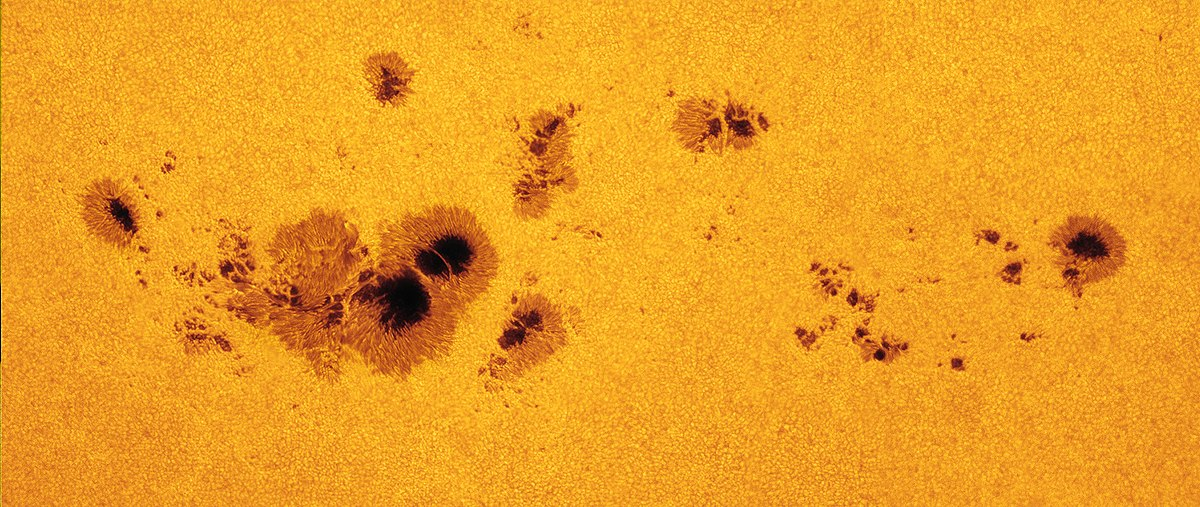
\includegraphics[width=1.0\textwidth, height=0.5\textwidth]{sunspot.jpg}
        \caption{A large group of sunspots stretching about 320,000 km (200,000 mi) across Image Credit: Wikimedia Commons}
        \label{fig:sunspot}
    \end{figure}
    \section{Applying MHD on Sunspots}
    Here, we'll consider a simple example which shows how we can use MHD to solve some physical problem. We'll take an example of \textbf{sunspot} and see how MHD can be used to explain the phenomenon. See the Figure \ref{fig:sunspot} for a picture of a sunspot. Sunspots are dark spots on the surface of the Sun which lasts typically for a number of days. They are magnetic regions on Sun with magnetic field strength thousands of times stronger than the Earth's magnetic field.

    Consider a sunspot as a verticle magnetic flux tube. The magnetic field lines are shown in Figure \ref{fig:flux-tube}. The magnetic fields $\mathbf{B_0}$ is verticle. $P_0$ and $T_0$ are the pressure and temperature inside the sunspot while $P_{E}$ and $T_{E}$ are the pressure and temperature outside the sunspot.\cite{article2}

    \begin{figure}[h]
        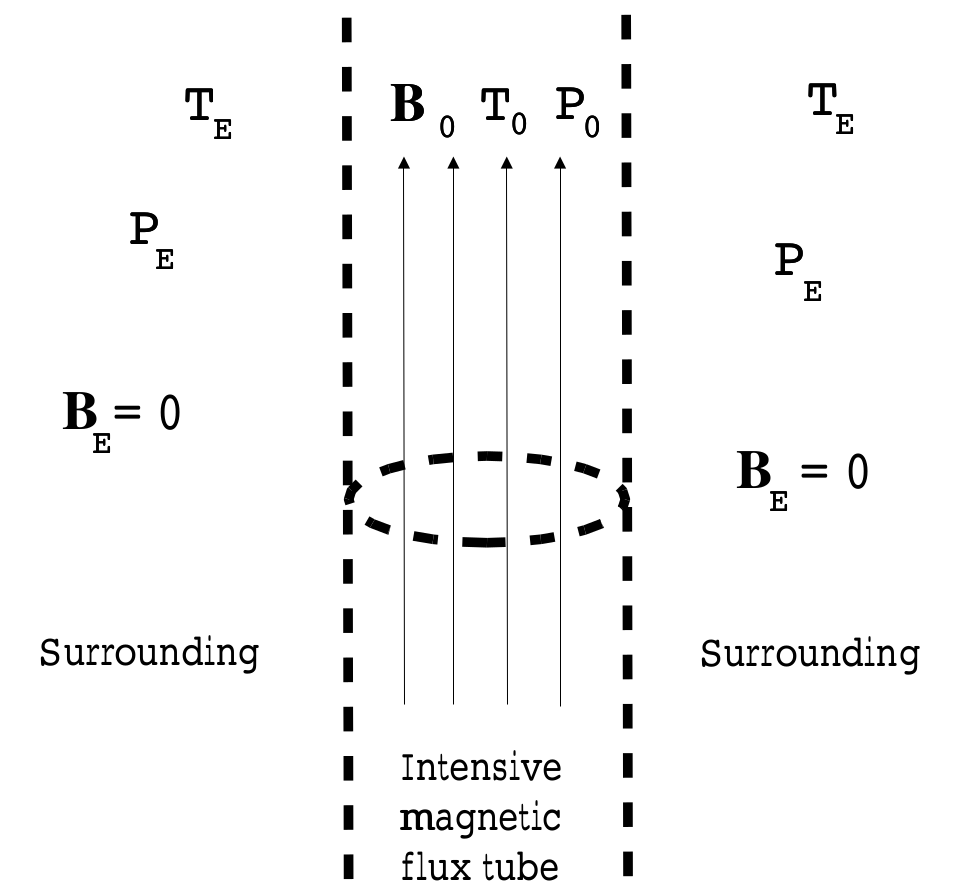
\includegraphics[width=1.0\textwidth, height=0.78\textwidth]{sunspot-tube.png}
        \caption{Vertical Magnetic Flux Tube}
        \label{fig:flux-tube}
    \end{figure}

    Since the magnetic field is straight, the magnetic tension force is zero. The magnetic pressure force is given by:
    \begin{equation}
        \nabla \left(P+{\frac {B^{2}}{2\mu _{0}}}\right) = 0
    \end{equation}
    This means that the pressure inside the sunspot is equal to the pressure outside the sunspot and hence
    \begin{equation}
        P_E = P_0 + \frac{B_0^2}{2\mu_0}
    \end{equation}
    We assume that the density is the same inside and outside the plasma, ie., $\rho_0 = \rho_E$. Dividing by them, the above equation becomes
    \begin{equation}
        \frac{P_E}{\rho_E} = \frac{P_0}{\rho_0} + \frac{B_0^2}{2\mu_0\rho_0}
    \end{equation}
    Next we use equations of state
    \begin{equation}
        P = 2\frac{k_B}{m}\rho T
    \end{equation}
    to obtain
    \begin{equation}
        \frac{2k_B}{m_i}T_E = \frac{2k_B}{m_i}T_0 + \frac{B_0^2}{2\mu_0\rho_0m_i}
    \end{equation}
    After simplifying, this gives:
    \begin{equation}\label{eq:sunspot-temp}
        \frac{T_E}{T_0} = 1 - \frac{B_0^2}{2\mu_0P_E}
    \end{equation}
    This means that in a sunspot $T_E>T_0$. This is indeed the case. Temperatures in the dark centers of sunspots may drop to about 3700K compared to the 5800K of the surrounding photosphere.

    \section{Non Linearty}
    \subsection{Why Non Linearty?}
    Linear MHD does not give answers to a lot of questions. For example, we saw that MHD is quite good at stability theory. However, it does not answer to the question that what happens to the equilibrium solutions if a weak perturbation is applied to it. Do they relax in a neighbouring equilibrium or oscillate about the equilibrium state? This question can be answered by non linear theory. What's more, linear instability theory does not allow an estimate of the final extent of the unstable dynamics.

    Hence it is necessary to leave the linear regime and study the non linear dynamics of the system. However, this means that even simple systems will become complicated. Hence nonlinear MHD studies are limited to object just a qualitative understanding in the simplest possible geometry while linear MHD can be used to deal quantitatively with more geometrically complicated systems. Usually, this is done by using numerical methods. We also make some simplification to the ideal MHD equations \ref{eq:mhd} to make them more tractable.\cite{nonlinear-mhd-book}

    \subsection{Reduced MHD Equations}
    The original MHD equation (Equation \ref{eq:mhd}) contain seven independent dynamic variables: hree velocity components, Two magnetic field components as $\nabla \cdot \mathbf{B} = 0$, Density and Pressure.
    % \begin{enumerate}
    %     \item Three velocity components
    %     \item Two magnetic field components as $\nabla \cdot \mathbf{B} = 0$
    %     \item Density
    %     \item Pressure
    % \end{enumerate}
    However, assuming incompressiblity and homogeneous density, we can reduce the number of dynamic variables to four, two velocity components (As $\nabla \cdot \mathbf{v} = 0$) and two magnetic field components. Pressure is now a functions of $\mathbf{v}$ and $\mathbf{B}$ while density is a constant. This is called the \textbf{reduced MHD equations}. The complete equations are\cite{article3}:
    \begin{align}\label{eq:reduced-mhd-1}
        \begin{split}
            \frac{\partial \psi}{\partial t} + \mathbf{v_\perp}\cdot \nabla \psi&=D_{\eta}\nabla^2\psi - B_{z0}\frac{\partial \phi}{\partial z}\\
            \rho_0\left(\frac{\partial \omega_z}{\partial t} + \mathbf{v_\perp}\cdot \nabla \omega_z \right) & = \mathbf{B}\cdot \nabla (J_z)\\
        \end{split}
    \end{align}
    With
    \begin{align}\label{eq:reduced-mhd-2}
        \begin{split}
            \omega_z &= \nabla_\perp^2\phi\\
            \frac{4\pi}{c}J_z &= \nabla^2 \psi\\
            \mathbf{v_\perp} &= \mathbf{\hat{z}}\times \nabla \phi\\
        \end{split}
    \end{align}
    % \subsection{Work Done Using Non Linear MHD}
    % A lot of work has been done using non linear MHD. Most of them are simulations as non linear MHD is very difficult to solve analytically. For example: "Linear and nonlinear particle-magnetohydrodynamic simulations of the toroidal Alfvén eigenmode" \cite{nonlinear2}

    \section{Whistler: The Hall MHD}
    In ideal MHD, there are only 3 types of waves: Alfv\'en wave, fast magnetosonic wave and slow magnetosonic wave. However, if
    we include the Hall term, we will get two more waves: whistler wave and the ion cyclotron wave.\cite{article4} To get a dispersion relation for whistler, we'll start by normalizing MHD equations with generalized Ohm's law.

    \subsection{Ohm's Law and Normalization}
    Taking only the resistive and Hall term in the generalized Ohm's law, we get:
    \begin{equation}
        \mathbf{E} + \mathbf{v\times B} = \eta \mathbf{J} + \frac{1}{ne}\mathbf{J\times B}
    \end{equation}
    Taking curl of both sides and using Faraday equation, this gives:
    \begin{equation}\label{eq:ohm1}
        \frac{\partial \mathbf{B}}{\partial t} = \nabla \times \left(\mathbf{v\times B}\right)- \nabla \times (\eta \mathbf{J}) -\nabla \times \left(\frac{1}{ne}\mathbf{J\times B}\right)
    \end{equation}
    This equation can be normalized by defining Alfv\'en speed $V_A = \frac{B}{\sqrt{\mu_0 n m_i}}$, Alfv\'en time $\tau_A = \frac{L}{V_A}$ and $L$ being the length of Normalization. Using these, the Equation \ref{eq:ohm1} can be written in normalized form as:
    \begin{equation}\label{eq:ohm-normal}
        \frac{\partial \mathbf{B}}{\partial t} = \nabla \times \left(\mathbf{v\times B}\right)- \frac{1}{S}\nabla \times \mathbf{J} -\frac{d_i}{L}\nabla \times \left(\frac{\mathbf{J\times B}}{n}\right)
    \end{equation}
    Where $d_i$ is the ion inertial length and $S$ is the Lundquist number defined as:
    \begin{align}
        \begin{split}
            \mathbf{J} &= \nabla \times \mathbf{B}\\
            d_i = \frac{V_A}{\omega_{ci}} &= \sqrt{\frac{m_i}{\mu_0 n e^2}}\\
            S = \frac{LV_A\mu_0}{\eta}
        \end{split}
    \end{align}

    Similarly, by help of $nm_iV_A^2$ to normalize pressure, the normalized form of the momentum equation is:
    \begin{eqnarray}\label{eq:momentum-normal}
        n\left(\frac{\partial \mathbf{v}}{\partial t}+\mathbf{v} \cdot \nabla \mathbf{u} \right) = -\nabla p + \mathbf{J\times B}
    \end{eqnarray}

    \subsection{Whistler Wave}
    As stated earlier, when Hall term is added to the MHD equations, we get two more waves one of them being the whistler wave. To get the dispersion relation, we'll start by the normalized equations \ref{eq:ohm-normal} and \ref{eq:momentum-normal}. Ignoring the resistive term, assuming a uniform background fields $\mathbf{B_0} = 1, \: n_0 = 1 \: \text{and } \mathbf{v_0} = 0$ and assuming the perturbation to be incompressible so that $n_1=0$ and $\mathbf{k \cdot v_1} = 0$. Next, we'll take curl of the momentum equation \ref{eq:momentum-normal} and consider only the normal term. This gives:
    \begin{equation}
        \frac{\partial}{\partial t}(\nabla \times \mathbf{v_1}) = \nabla \times (\mathbf{J_1\times B_0})
    \end{equation}
    Similarly, taking the linear form of the Ohm's equation \ref{eq:ohm-normal}:
    \begin{equation}
        \frac{\partial \mathbf{B_1}}{\partial t} = \nabla \times \left(\mathbf{v_1\times B_0}\right)-d_i\nabla \times \left(\mathbf{J_1\times B_0}\right)
    \end{equation}
    Now, replacing $\frac{\partial}{\partial t}$ with $-i\omega$ and $\nabla$ with $\mathbf{k}$ and then eliminating $B_1$ gives:
    \begin{equation}\label{eq:el1}
        \left[\omega - \frac{(\mathbf{k \cdot B_0})^2}{\omega} \right](\mathbf{k \times v_1}) + id_1k^2(\mathbf{k \cdot B_0})\mathbf{v_1} = 0
    \end{equation}
    While taking curl of the above equation gives:
    \begin{equation}\label{eq:el2}
        -k^2\left[\omega - \frac{(\mathbf{k \cdot B_0})^2}{\omega} \right]\mathbf{v_1} + id_1k^2(\mathbf{k \cdot B_0})(\mathbf{k \times v_1}) = 0
    \end{equation}

    Combining Equations \ref{eq:el1} and \ref{eq:el2} and setting the determinant of the coefficients to zero, we get the dispersion relation:
    \begin{equation}
        \left[\omega - \frac{(\mathbf{k \cdot B_0})^2}{\omega} \right]^2 = \left[kd_i(\mathbf{k \cdot B_0})\right]^2
    \end{equation}
    Taking the square root gives two waves, the dispersion relations are:
    \begin{equation}\label{eq:whistler}
        \omega_{\pm} = \frac{\sqrt{(kd_i)^2+4}\pm kd_i}{2}(\mathbf{k \cdot V_A})
    \end{equation}
    Note that in above equation, we have normalized the quantites to the real quantites. Equation \ref{eq:whistler} is the dispersion relation for the whistler wave. See the Figure \ref{fig:whistler} for the dispersion curve. The $\omega_+$ is right-hand polarized while the $\omega_-$ is left-hand polarized.

    \begin{figure}[h]
        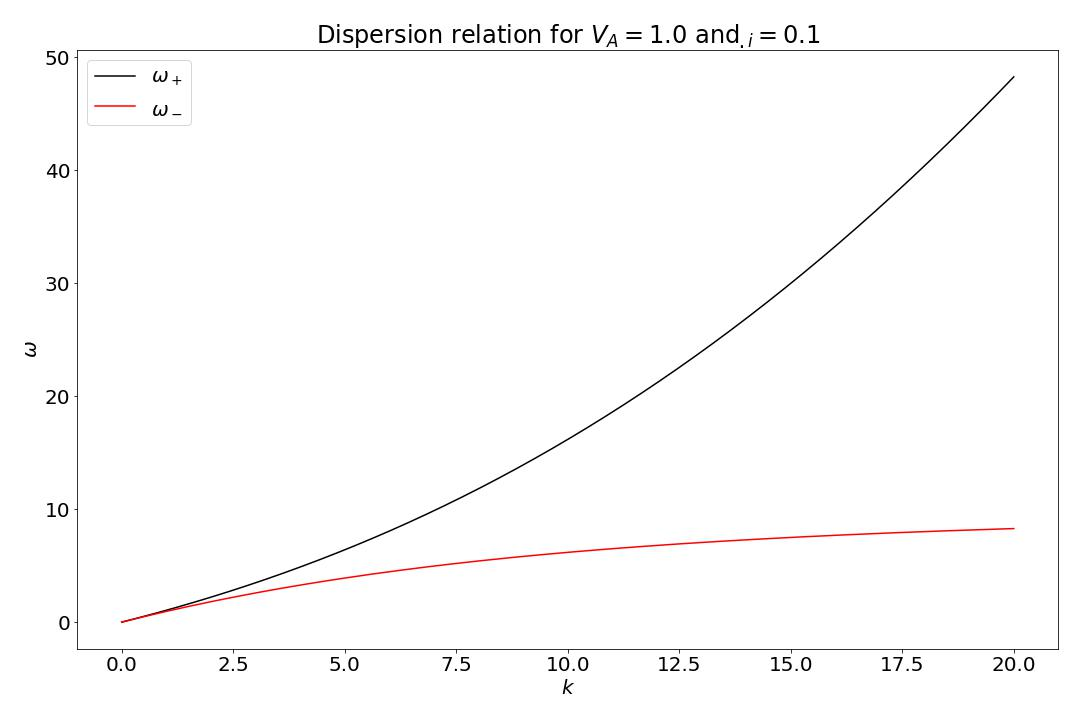
\includegraphics[width=1.0\textwidth, height=0.78\textwidth]{dispersion.jpg}
        \caption{Dispersion Relation for Whistler Waves}
        \label{fig:whistler}
    \end{figure}
    \section{Conclusion}
    We started by discussing history and basic introduction of MHD followed by assumptions made by the model along with its usefulness and limitations. After that, we wrote the set of seven equations which are needed to solve simultaneously. We also talked about what is \textit{ideal} in the ideal MHD. This was followed by a simple example where we used MHD to show that the temperature of sunspots (Equation \ref{eq:sunspot-temp}) are lower than its surrounding. Then we proceded to show that linear MHD is not always helpful and it is not able to answer a lot of questions. We talked about using nonlinearty to answer these questions and discussed the complications made by introducing nonlinearty as well as restrictions posed by this on physical systems in which we can use this. It turned out that numerical approach will be much more fruitful for non linear case. We also talked about the reduced MHD equations \ref{eq:reduced-mhd-1} and \ref{eq:reduced-mhd-2} which is easier to tackle.

    Finally, we saw that including Hall effect in the MHD equations \ref{eq:mhd} results in generation of whistler mode. We normalized and linearized the Ohm's equation \ref{eq:ohm-normal} and the momentum equation \ref{eq:momentum-normal} to get the dispersion relation \ref{eq:whistler} for the whistler wave. We saw that there are two waves in the mode, one right and other left polarized. We also made a plot (Figure \ref{fig:whistler}) of the dispersion curve using \textcolor{cyan}{matplotlib} and \textcolor{cyan}{Python}.
    % \newpage
    \printbibliography
\end{changemargin}
\end{document}